\documentclass{tufte-handout}
\usepackage{amsmath}
\pagestyle{empty}
\usepackage[utf8]{inputenc}
\usepackage{mathpazo}
\usepackage{microtype}

\usepackage{tikz}
\usetikzlibrary{matrix}
\usetikzlibrary{chains}
\usetikzlibrary{decorations}

\title{Stable Matching}
\author{Thore Husfeldt}

\begin{document}

\maketitle

\subsection{Description}
Implement Gale–Shapley’s algorithm for stable matching and run it on several test inputs.

\begin{marginfigure}
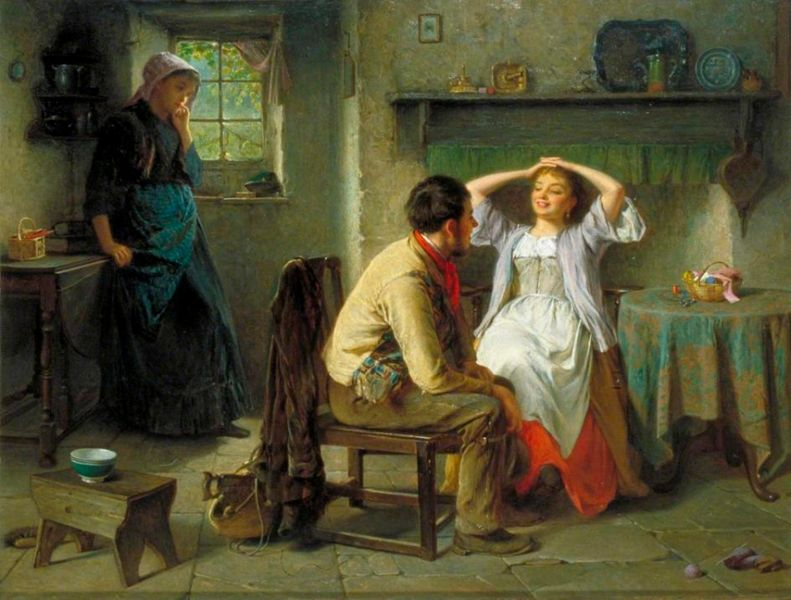
\includegraphics[width=2in]{791px-Jealousy_and_Flirtation.jpg}
\caption{\emph{Jealousy and Flirtation} (1874) by Haynes King (1831-1904).
Source: Wikimedia Commons. Public domain.}
\end{marginfigure}

\subsection{Requirements}
Your programme has to take its input either from standard input (STDIN) or from a specified file.
It has to write to standard output (STDOUT).
Assuming all the files are in the right place and you wrote your code in Java, you must be able to run the programme from the command line with at least one of the following two commands:
\begin{verbatim}
  % java GS < sm-kt-p-4.in
  % java GS sm-kt-p-4.in
\end{verbatim}

\paragraph{Correctness}
The course data file directory contains a number of pairs of files called “{\tt sm-*-in.txt}” and “{\tt sm-*-out.txt}” that contain matching input and expected output.
Your solution must be consistent with these files.
(The ordering of your output makes no matter.)
Your code has to be as clear and crisp as possible.
Your solution must run in time $O(n^2)$, where $n$ is the number of women (and men).
In particular, this means that your solution must be able to handle the pairwise comparison of two men in a woman’s list of preferences in constant time.
Section [KT, 2.3] explains how to do this.

\section{Questions}

\begin{description}
  \item[What about coding paradigms?]
    I don’t much care.
    You can follow the book and make an array-based solution, where people are basically integers that are used as indices into various arrays.
    You can also try for an object-oriented approach where people are objects (or even make Person is an abstract class or an interface, implemented by Man and Woman), and the data structures use a standard collections package.
    Maybe there’s even a beatiful functional solution.
  \item[Style?]
    Your code should be as neat as you can make it.
    Don’t declare variables or fields or methods that you never use.
  \item[What about documentation?]
    I don’t much care.
    I’d much rather have your code be as short and sweet as possible, instead of full of comments.
    Especially, don’t waste time explaining the algorithm---the expected audience has read the book!
\end{description}

\section{Tips}

 
Algorithmically, this is supposed to be an easy exercise.
The algorithm is simple and spelt out in detail on p. 6 in the book, and many implementation issues are addressed in section 2.3.
However, what is probably going to take you a lot of time is reading the input, especially if you haven’t done that kind of thing before.
I suggest the following:
\begin{enumerate}
  \item First, hard-code the input, in a convenient data structure, while
you get the algorithm to work.
This will allow you to change your mind about how the data structures should look.
Only when everything seems to look OK, read (and parse!) your input from standard input.
\item If you do this in Java, learn {\tt java.util.Scanner}.
  You want something like {\tt Scanner SC = new Scanner(System.in)}.
\item When debugging, don’t throw away your test cases!
  Instead, make additional input–output file pairs.
\item Write another program that runs your Gale--Shapley implementation on all test files (both the ones I have made and those you may have produced during debugging) and checks them against the corresponding output files.
  This requires nontrivial file operations (opening matching filenames, reading directories, comparing files), and Java may not be the best language to do that in.
  (You could learn Perl or shell scripting.)
\item What annoyed me most about input are the indices.
  In my array-based solution, after changing my minds a million times, I settled for indexing the men by $\{0,\ldots,n-1.$ and the women $\{0,\ldots,n-1\}$.
    This made the parsing stage slightly more complicated, because the input file uses a different convention, but cleaned up the rest of my code a lot.
  \end{enumerate}
\subsection{Deliverables}

\begin{enumerate}
  \item The source code for your implementation
  \item A report in PDF.
  Use the report skeleton in the {\tt doc} directory.
  \end{enumerate}

\end{document}
